\documentclass{article}

% Language setting
% Replace `english' with e.g. `spanish' to change the document language
\usepackage[french]{babel}
\usepackage[fleqn]{amsmath} % Aligner les équations à gauche


% Set page size and margins
% Replace `letterpaper' with`a4paper' for UK/EU standard size
\usepackage[letterpaper,top=2cm,bottom=2cm,left=3cm,right=3cm,marginparwidth=1.75cm]{geometry}

% Useful packages

\usepackage{amsmath}
\usepackage{amssymb}
\usepackage{bbold}

\usepackage{graphicx}
\usepackage{subcaption}
\usepackage[colorlinks=true, allcolors=blue]{hyperref}

\title{TD 4 - Calcul Vectoriel}
\author{IPESUP - PC }
\date{2/10/2024}

\begin{document}
\maketitle

\section{Rappels de cours}

\textbf{Définitions:} \\[0.2cm]

Soit $\vec{f}$ un champ vectoriel et $g$ un champ scalaire, tous les deux dans $\mathbb{R}^3$. On définit les opérateurs suivants: 

\begin{enumerate}
  \item Gradient : $\vec{grad}(g) = \vec{\nabla} g$ = $\left( \begin{matrix}
    \frac{\partial g}{\partial x}  \\[0.1cm]
    \frac{\partial g}{\partial y}  \\[0.1cm]
    \frac{\partial g}{\partial z} \\[0.2cm]
    \end{matrix}
    \right) $

  \item Divergence : div($\vec{f}$) = \(\vec{\nabla} \cdot \vec{f}\) = \(\frac{\partial f_x}{\partial x} + \frac{\partial f_y}{\partial y} + \frac{\partial f_z}{\partial z}\) \\[0.2cm]
  \item Rotationnel : $\vec{rot}$($\vec{f}$) = \(\vec{\nabla} \times \vec{f}\) = 
    $ \left( \begin{matrix}
    \frac{\partial f_z}{\partial y} - \frac{\partial f_y}{\partial z}  \\[0.1cm]
    \frac{\partial f_x}{\partial z} - \frac{\partial f_z}{\partial x}  \\[0.1cm]
    \frac{\partial f_y}{\partial x} - \frac{\partial f_x}{\partial y} \\[0.1cm]
  

  \end{matrix} \right) $ 
  \item Laplacien scalaire : $\Delta g =  \vec{\nabla}^2 g = \frac{\partial^2 g}{\partial x^2} + \frac{\partial^2 g}{\partial y^2} + \frac{\partial^2 g}{\partial z^2}$
  \item Laplacien vectoriel : $\vec{\Delta} \vec{f} = \vec{\nabla}^2 \vec{f} =
   \left( \begin{matrix}
    \Delta  f_x  \\[0.1cm]
    \Delta  f_y  \\[0.1cm]
    \Delta  f_z \\[0.1cm]
    \end{matrix}  \right) $ 
\end{enumerate}



\textbf{Remarques:} \\[0.2cm]

\begin{itemize}
  \item div($\vec{f}$) et $\nabla^2 g$ sont des scalaires. 
  \item $\vec{rot}$($\vec{f}$), $\nabla^2 \vec{f}$ et $\vec{grad}$($\vec{f}$)  sont des vecteurs. 
  \item Tous ces opérateurs sont \textbf{linéaires}.
  \item Vous devez connaître les formules ci-dessus. Leurs expressions en coordonnées sphériques et cylindriques ne sont \textbf{pas} à connaître et vous seront redonnées à chaque fois.
  \item L'opérateur nabla permet de retrouver les expressions des opérateurs ci-dessus en coordonnées cartésiennes uniquement.  \\[0.2cm]
\end{itemize}

\textbf{Formules en coordonnées cylindriques:} \\[0.2cm]  

\begin{itemize}
  \item $\vec{grad} (g) = \frac{\partial g}{\partial r} \vec{e}_r + \frac{1}{r} \frac{\partial g}{\partial \theta} \vec{e}_\theta + \frac{\partial g}{\partial z} \vec{e}_z$
  \item div($\vec{f}$) $= \frac{1}{r} \frac{\partial}{\partial r}(r f_r) + \frac{1}{r} \frac{\partial f_\theta}{\partial \theta} + \frac{\partial f_z}{\partial z}$
  \item $\vec{rot}(\vec{f}) = \left( \frac{1}{r} \frac{\partial f_z}{\partial \theta} - \frac{\partial f_\theta}{\partial z} \right) \vec{e}_r 
  + \left( \frac{\partial f_r}{\partial z} - \frac{\partial f_z}{\partial r} \right) \vec{e}_\theta 
  + \frac{1}{r} \left( \frac{\partial}{\partial r}(r f_\theta) - \frac{\partial f_r}{\partial \theta} \right) \vec{e}_z $ \\[1cm]
\end{itemize}

\textbf{Formules en coordonnées sphériques:} \\[0.2cm]
\begin{itemize}
  \item $\vec{grad} (g) = \frac{\partial g}{\partial r} \vec{e}_r + \frac{1}{r} \frac{\partial g}{\partial \theta} \vec{e}_\theta + \frac{1}{r \sin \theta} \frac{\partial g}{\partial \phi} \vec{e}_\phi$
  \item div($\vec{f}$) $=\frac{1}{r^2} \frac{\partial}{\partial r}(r^2 f_r) + \frac{1}{r \sin \theta} \frac{\partial}{\partial \theta}(\sin \theta f_\theta) + \frac{1}{r \sin \theta} \frac{\partial f_\phi}{\partial \phi}$
  \item $\vec{rot}(\vec{f})  = \frac{1}{r \sin \theta} \left( \frac{\partial}{\partial \theta}(f_\phi \sin \theta) - \frac{\partial f_\theta}{\partial \phi} \right) \vec{e}_r
  + \frac{1}{r} \left( \frac{1}{\sin \theta} \frac{\partial f_r}{\partial \phi} - \frac{\partial}{\partial r}(r f_\phi) \right) \vec{e}_\theta
  + \frac{1}{r} \left( \frac{\partial}{\partial r}(r f_\theta) - \frac{\partial f_r}{\partial \theta} \right) \vec{e}_\phi $ \\[1cm]
  

\end{itemize}

\textbf{Quelques identités utiles:} \\[0.2cm]
\begin{itemize}
  \item $div(\vec{grad}(g)) = \Delta g  $
  \item $div(\vec{rot}(\vec{f})) = 0$
  \item $\vec{rot}(\vec{grad}(g)) = \vec{0}$
  \item $ \vec{rot}(\vec{rot}(\vec{f})) = \vec{grad}(div(\vec{f})) - \vec{\Delta} \vec{f}$
  \item Champ dérivant d'un potentiel: $  \vec{rot}(\vec{f}) = \vec{0} \Leftrightarrow   \exists g :   \vec{f} = \vec{grad}(g)  $ \\[0.3cm]

\end{itemize}


\textbf{Formule de Stokes:} \\[0.2cm]

Soit $\vec{f}$ un champ vectoriel, $\Gamma$ un contour \textbf{fermé}  orienté dans le sens direct et $S$ une surface quelconque, \textbf{orientée} par le vecteur normal $\vec{n}$ (règle de la main droite) et s'appuyant sur $\Gamma$. On a:\\[0.15cm]
$\boxed{ \oint_\Gamma \vec{f} \cdot d\vec{l} = \iint_S \vec{rot}(\vec{f}) \cdot d\vec{S}}$\\[0.3cm]


\textbf{Formule d'Ostrogradski:} \\[0.2cm]

Soit $S$ une surface fermée de normale $\vec{n}_{ext}$ orientée vers \textbf{l'extérieur}. Soit $\vec{f}$ un champ vectoriel. On a: \\[0.15cm]
$\boxed{ \iint_S \vec{f} \cdot d\vec{S} = \iiint_V div(\vec{f}) dV}$\\[0.3cm]

\textbf{Remarque:} \\[0.2cm]

En toute rigueur, pour le théorème de Stokes, il faut que $\Gamma$ soit de classe $\mathcal{C}^1$ par morceaux, que $\vec{f}$ ait des dérivées partielles de premier ordre continues et que $S$ soit une surface régulière. 
Pour le théorème d'Ostrogradski, il faut que $S$ soit une surface différentiable par morceaux, que $V$ soit compact et que $\vec{f}$ soit continûment différentiable. 
En pratique, on ne vérifiera \textbf{JAMAIS} ces conditions. \\[0.5cm]



\textbf{Anecdote} (sur la lumière, il n'existe pas d'anecdotes rigolotes sur le calcul vectoriel):  \\[0.1cm]
La diffraction de la lumière a été théorisée par Augustin Fresnel, un physicien français. En 1819, lors d'un concours organisé par l'Académie des sciences pour résoudre la question de la nature de la lumière, Fresnel soumit une explication mathématique détaillée de la diffraction.

L'un des juges, Siméon Denis Poisson, un fervent défenseur de la théorie corpusculaire de Newton, tenta de réfuter Fresnel en affirmant que son modèle ondulatoire menait à une prédiction absurde : si la lumière se comportait comme une onde, alors lorsqu'un disque opaque est placé devant une source lumineuse ponctuelle, un point lumineux devrait apparaître au centre de l'ombre projetée. C'était tellement contre-intuitif que Poisson pensait que cela discréditerait Fresnel.

Cependant, lorsqu'un autre membre du comité, François Arago, réalisa l'expérience en laboratoire, il observa effectivement ce point lumineux central, maintenant appelé tache de Poisson. Cette observation a validé la théorie ondulatoire et discrédité l'argument de Poisson.


\section{Exercice 1}

\begin{itemize}
  \item Retrouver la formule du gradient en coordonnées sphériques et cylindriques.
  \item Reprouver les 4 premières identités utiles par calcul vectoriel (avec $\vec{\nabla})$ et en coordonnées cartésiennes.
\end{itemize}

\section{Exercice 2}

Soit $\vec{E}$ un champ vectoriel défini sur $\mathbb{R}^3$. On ne sait rien sur ce champ, mais on mesure sa divergence. On a : \\

$ div(\vec{E}(x, y, z)) = \mathbb{1}_{(0,0,0)}$ \\
\begin{itemize}
  \item Par des arguments de symétrie, montrer que $\vec{E}$ est parallèle à $\vec{e_r}$.
  \item Par des arguments d'invariance, montrer que $\vec{E}$ ne dépend pas de $\theta$ ni de $\phi$.
  \item En utilisant le théorème de Stokes, calculer $\vec{E}$ en tout point de l'espace.
\end{itemize}



\section{Mines PC 2013 Physique 1}
Questions 19 à 25. \\[3cm]


\begin{figure}[h!]
  \centering
  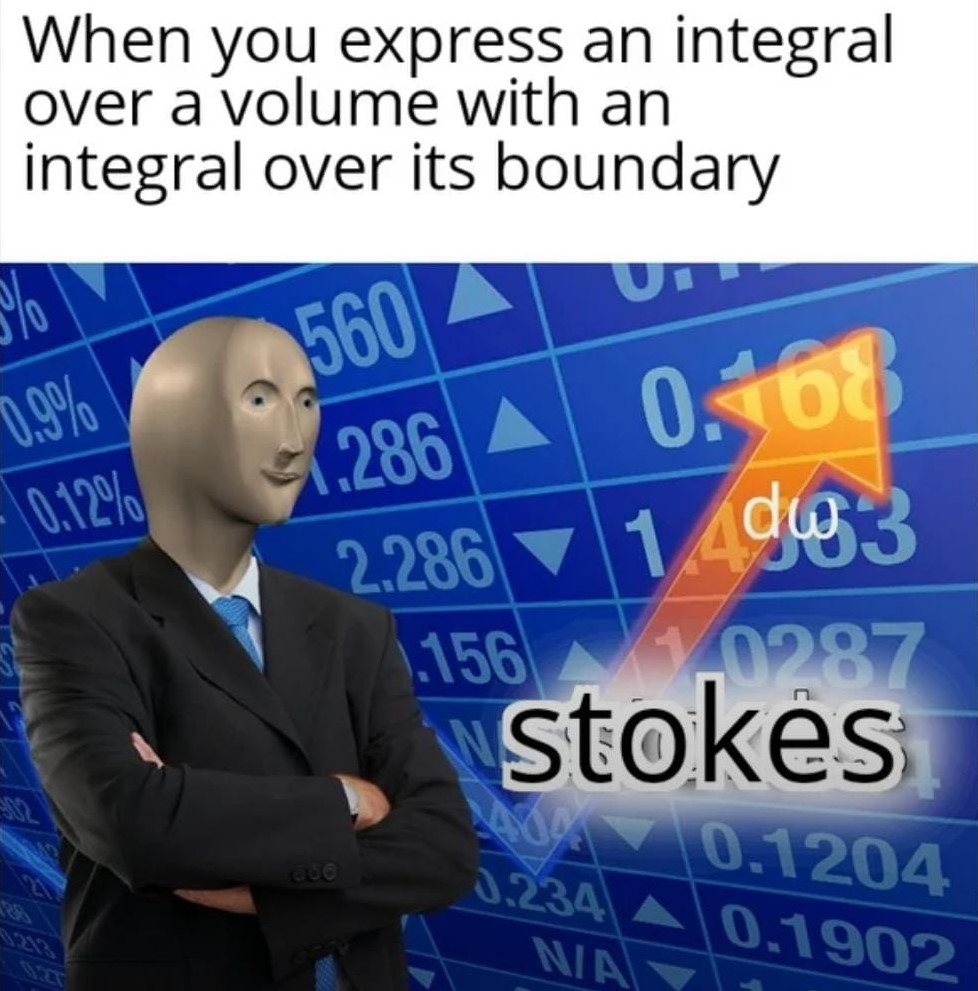
\includegraphics[width=0.4\textwidth]{stokes.jpg}
\end{figure}

\end{document}

